%トランジスタ等素子の説明
\chapter{各種素子の動作原理}
\section{半導体}
半導体とは、絶縁体に違う種類の不純物をドープすることによって導電性を持たせた材料である。代表的な半導体材料としてシリコン(Si)やゲルマニウム(Ge)がある。
半導体はドープする不純物の種類によって、p型半導体とn型半導体に分類される。
最外殻電子が4個のシリコンに、最外殻電子が5個のリン(P)などの不純物をドープすると、余分な電子が導電に寄与するためn型半導体となる。
一方、最外殻電子が3個のホウ素(B)などの不純物をドープすると、電子が不足するため正孔が導電に寄与し、p型半導体となる。



\section{ダイオードの動作原理}
ダイオードは図\ref{fig:diode_section}のようにp型半導体とn型半導体を接合して作られた素子である。
\begin{figure}[htbp]
    \centering
    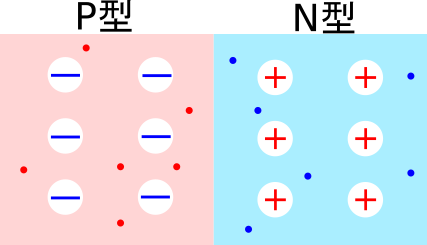
\includegraphics[width=0.5\textwidth]{graphit/diode.png}
    \caption{ダイオードの断面図}
    \label{fig:diode_section}
\end{figure}
ここで、図\ref{fig:diode_section}のP型のほうにある小さい丸は正孔を、N型のほうにある小さい丸は電子を表している。
また、P型のほうにある大きい丸は正孔が移動することによってできた負の固定電荷を、N型のほうにある大きい丸は自由電子が移動することによってできた正の固定電荷を表している。

これらの自由電子と正孔は自由に動くことができるため勝手に拡散し、P型半導体とN型半導体との境界付近で、自由電子と正孔が再結合する。(図\ref{fig:diode_diffusion}参照)
\begin{figure}[htbp]
    \begin{minipage}
        {0.45\hsize}
        \centering
        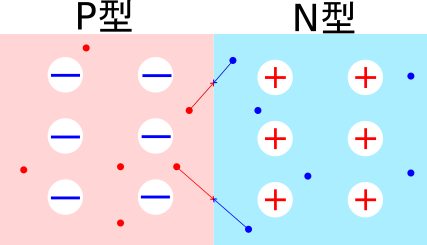
\includegraphics[width=0.8\textwidth]{graphit/diode_extinction.png}
        \caption{ダイオードにおける自由電子と正孔の再結合}
        \label{fig:diode_diffusion}
    \end{minipage}
    \begin{minipage}
        {0.45\hsize}
        \centering
        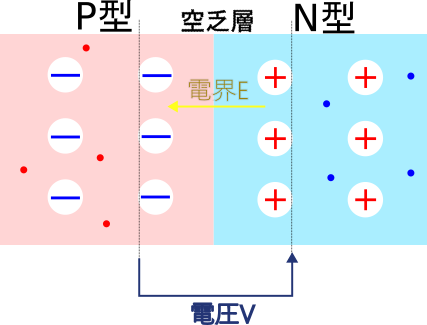
\includegraphics[width=0.8\textwidth]{graphit/diode_depletion.png}
        \caption{ダイオードにおける空乏層の形成}
        \label{fig:diode_depletion}
    \end{minipage}
\end{figure}

この再結合が進むと、境界付近には自由電子と正孔がいなくなり、固定電荷だけが残る領域ができる。この領域を空乏層と呼ぶ。(図\ref{fig:diode_depletion}参照)

この領域には固定電荷が残っていいるため、これによる電界がN型半導体側からP型半導体側に向かって発生する。この電界は自由電子と正孔の拡散を妨げる向きに働くため、自由電子と正孔の拡散が止まり、
空乏層の拡大も止まる。ここの電位差を拡散電位(built-in potential)と呼び、P型半導体とN型半導体とのフェルミ準位の差に等しい。

ここで、電圧をN側を正として印加することを考えてみると、空乏層と同じ方向の電界が発生するため、空乏層を大きくする方法に働き、電流は少ししか流れない。
ここで電流が少ししか流れないといったが、実は、P型半導体にはメインキャリアの正孔の他に少数キャリアの電子が存在し、N型半導体には少数キャリアの正孔が存在する。
これらは熱励起などによって生成されるため、少数キャリアは常に存在する。この少数キャリアが空乏層を通過することによって、逆方向にもわずかな電流が流れる。

次に、電圧をP側を正として印加してみると、空乏層と逆方向の電界が発生するため、空乏層を小さくする方向に働き、自由電子と正孔が空乏層を通過しやすくなる。
その結果、大きな電流が流れるようになる。このように、ダイオードは一方向にのみ大きな電流を流す素子である。
なお、P型半導体側をアノード、N型半導体側をカソードと呼ぶ。

ダイオードの電圧-電流特性は
\begin{align}
    I_D = I_S \left\{ \exp{\left(\frac{eV}{k_bT}\right)} - 1 \right\}
\end{align}
という風に表される。(図\ref{fig:diode_specific})ここで、$I_D$はダイオード電流、$I_S$は逆方向飽和電流、$e$は素電荷、$V$はダイオードにかかる電圧、$k_b$はボルツマン定数、$T$は絶対温度である。
室温付近では大体$V_T = k_bT/e \approx 26mV$である。
\begin{figure}[htbp]
    \centering
    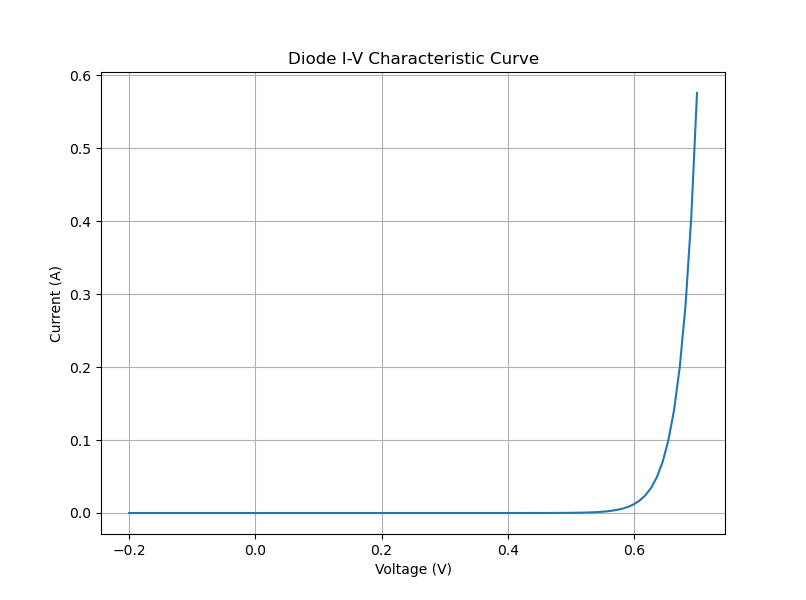
\includegraphics[width=0.8\textwidth]{diode_IV.png}
    \caption{ダイオードの電圧-電流特性($I_S = 10^{-12}$A,$V_T = 25.85$mV)}
    \label{fig:diode_specific}
\end{figure}
\newpage

図\ref{fig:diode_specific}からわかるように、ダイオードは順方向に約0.7V以上の電圧がかかると急激に電流が流れ始める特性を持っている。

% \subsection{ダイオードのコラム}
% ツェナー降伏とかアノード・カソードとか真空管とか


\section{バイポーラトランジスタの動作原理}
バイポーラトランジスタ(以下BJT)は、3つの半導体領域を接合して作られた素子である。NPN型とPNP型の2種類があるが、ここではNPN型について説明する。 図\ref{fig:bjt_section}にBJTの断面図を示す。
\begin{figure}[htbp]
    \centering
    \includegraphics[width=0.5\textwidth]{graphit/bjt.png}
    \caption{バイポーラトランジスタの断面図}
    \label{fig:bjt_section}
\end{figure}
BJTはエミッタ(E)、ベース(B)、コレクタ(C)の3つの端子を持つ。エミッタはn型半導体、ベースはp型半導体、コレクタはn型半導体で構成されているが、コレクタのn型半導体のドープ濃度はエミッタのn型半導体のドープ濃度よりも低い。

N型半導体とP型半導体の接合部にはダイオードと同じようにそれぞれ空乏層が形成される。

ここでエミッタからベースに電圧を印加し、ベース電流$I_B$を流すと、エミッタベース間のエミッタベース間の空乏層がつぶれ、エミッタからベースに向かって多数キャリアである電子が注入される。
ベースはp型半導体であるため、注入された電子は正孔と再結合するが、
ここでベースコレクタ間に電圧を印加すると、ベースが十分に薄い場合、エミッタからベースに向かっていた電子のほとんどはコレクタベース間の空乏層に存在する電界の影響を受けてコレクタに引き寄せられ、
コレクタ電流$I_C$として流れる。(図\ref{fig:bjt_operation}参照)
\begin{figure}[htbp]
    \centering
    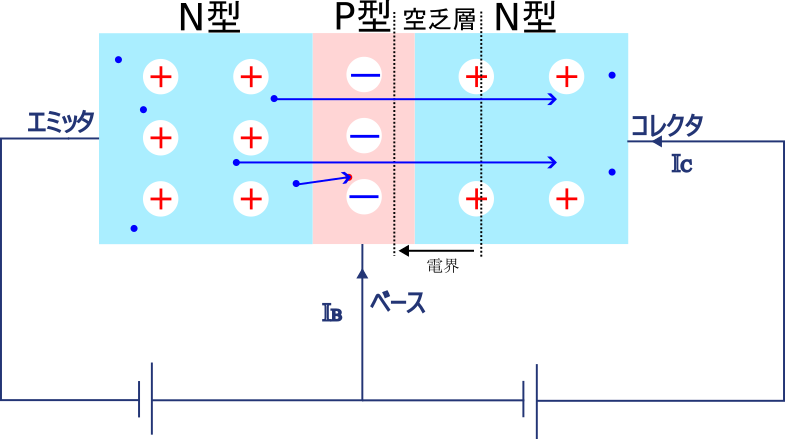
\includegraphics[width=0.5\textwidth]{graphit/bjt_operation.png}
    \caption{バイポーラトランジスタの動作原理}
    \label{fig:bjt_operation}
\end{figure}
このとき、エミッタ電流$I_E$はキルヒホッフの法則より、
\begin{align}
    I_E = I_B + I_C
\end{align}
である。また、エミッタから出発してコレクタに到達する電子の割合を$\alpha$とすると、
\begin{align}
    I_C = \alpha I_E
\end{align}
である。よって
\begin{align}
    I_C = \frac{\alpha}{1 - \alpha} I_B
\end{align}
となる。ここで、$\beta = \frac{\alpha}{1 - \alpha}$をBJTの電流増幅率と呼ぶ。
$\alpha$は0以上1未満の値をとるため、$\beta$は1以上の値をとる。通常、$\beta$は100程度の値をとるため、小さいベース電流$I_B$で大きなコレクタ電流$I_C$を制御することができる。

また、PNP型のBJTはNPN型BJTと同様の動作原理で動作する。

余談ではあるが、トランジスタのベースエミッタ間はN型半導体とP型半導体の接合部であるため、ダイオードと同様の電圧-電流特性を持つ。

\section{MOSFETの動作原理}
MOSFETは、金属酸化被膜電界効果トランジスタ(Metal-Oxide-Semiconductor Field Effect Transistor)の略であり、電界効果を利用して動作するトランジスタである。
MOSFETにはnチャネル型とpチャネル型の2種類があるが、ここではnチャネル型について説明する。図\ref{fig:mosfet_section}にMOSFETの断面図を示す。
\begin{figure}[htbp]
    \centering
    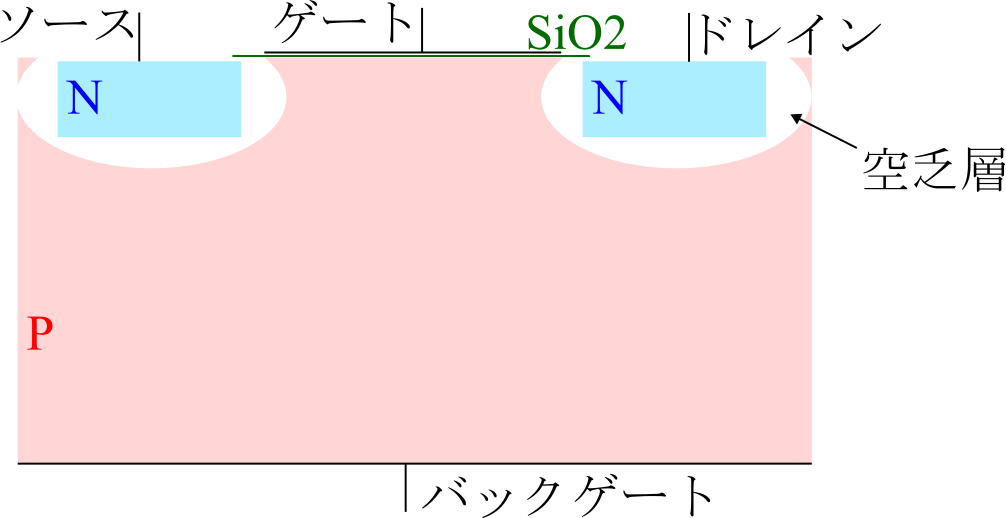
\includegraphics[width=0.5\textwidth]{graphit/mosfet.png}
    \caption{MOSFETの断面図}
    \label{fig:mosfet_section}
\end{figure}
MOSFETはソース(S)、ドレイン(D)、ゲート(G)、およびバックゲート(BG)の4つの端子を持つ。ソースとドレインはn型半導体で構成されている。
また、ゲートは絶縁膜(通常はSiO2)を介して基板に接続された金属電極である。
また、多くのMOSFETではバックゲート端子はソース端子に接続されている。
ここでゲートソース間に正の電圧$V_{GS}$を印加すると、基板内のp型半導体領域に電界が発生し、
p型半導体内部の少数キャリアである電子がゲート下に引き寄せられ、まるでn型としてふるまう反転層が形成される。
この反転層はソースとドレインを接続する導電チャネルとなるため、ドレインソース間に電圧$V_{DS}$を印加すると、ドレインからソースに向かって電子が流れ、ドレイン電流$I_D$が流れる。(図\ref{fig:mosfet_operation}参照)
\begin{figure}[htbp]
    \centering
    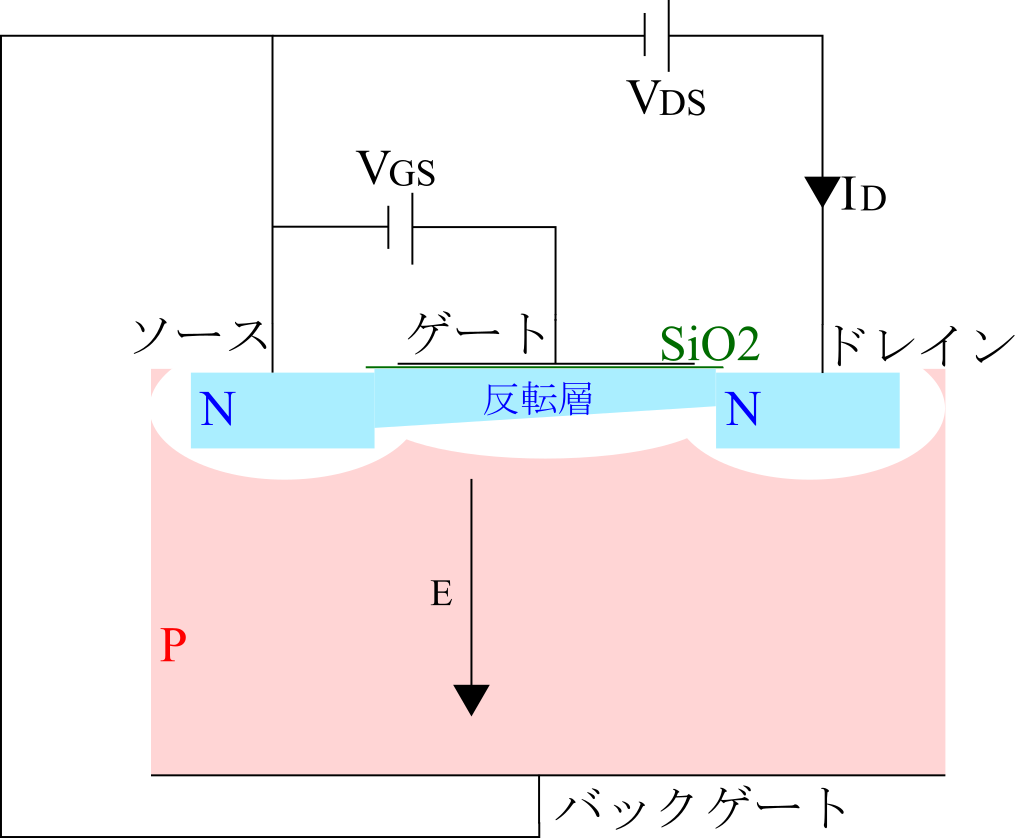
\includegraphics[width=0.5\textwidth]{graphit/mosfet_operation.png}
    \caption{MOSFETの動作原理}
    \label{fig:mosfet_operation}
\end{figure}
動作原理より、BJTと違って電流ではなくゲートソース間電圧$V_{GS}$によってドレイン電流$I_D$を制御することができる。

余談ではあるが、MOSFETのバックゲート=ソースとドレイン間にはpn接合が形成されているため、ダイオードと同様の電圧-電流特性を持つ。
この、バックゲート=ソースとドレイン間のpn接合を寄生ダイオード(ボディダイオード)と呼ぶ。


% \section{メカニカルリレーの動作原理}

\section{それぞれの回路での扱い方}
図\ref{fig:diode_cir},\ref{fig:bjt_cir},\ref{fig:mosfet_cir}にダイオード、BJT、MOSFETの回路記号を示す。
\begin{figure}[htbp]
    \begin{minipage}
        {0.3\hsize}
        \centering
        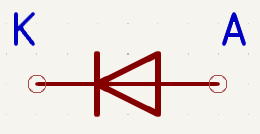
\includegraphics[width=0.5\textwidth]{graphit/diode_circuit.png}
        \caption{ダイオードの回路記号}
        \label{fig:diode_cir}
    \end{minipage}
    \begin{minipage}
        {0.3\hsize}
        \centering
        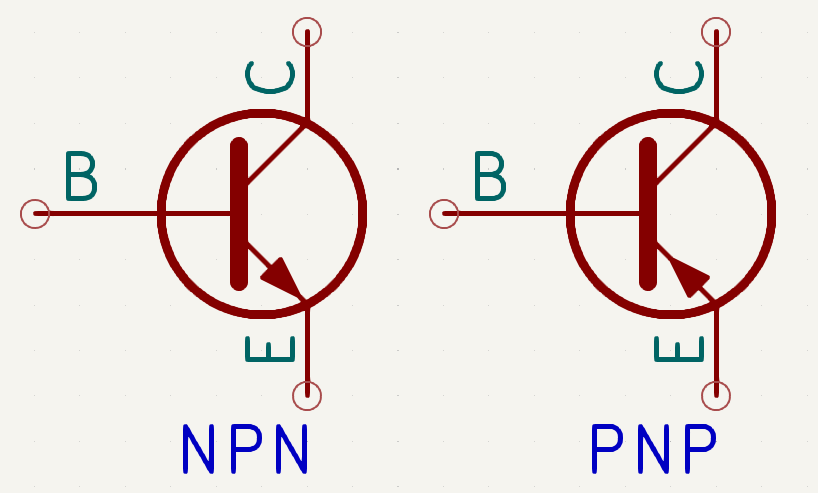
\includegraphics[width=0.8\textwidth]{graphit/bjt_circuit.png}
        \caption{BJTの回路記号}
        \label{fig:bjt_cir}
    \end{minipage}
    \begin{minipage}
        {0.3\hsize}
        \centering
        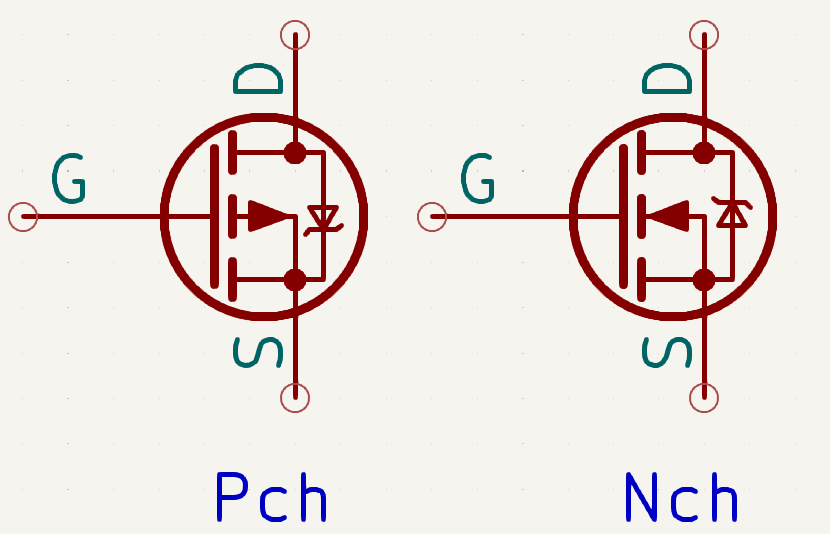
\includegraphics[width=0.8\textwidth]{graphit/mosfet_circuit.png}
        \caption{MOSFETの回路記号}
        \label{fig:mosfet_cir}
    \end{minipage}
\end{figure}
以下、この本ではこのように表記する。

各素子の論理回路での扱い方について説明する。
本来これらの素子は非線形素子であり、前章で習った基礎回路理論は通用しない。
しかし、論理回路では各素子をスイッチとして扱うことで、基礎回路理論を適用することができる。
\subsection{ダイオード}
ダイオードは順方向に電圧がかかると電流が流れ、逆方向に電圧がかかるとほとんど電流が流れない特性を持つ。
そのため、論理回路では順方向に閉じたスイッチ、逆方向に開いたスイッチとして扱う。
\subsection{バイポーラトランジスタ}
NPN型BJTはベースに十分な電流が流れるとコレクタからエミッタに大きな電流が流れ、ベースに電流が流れないとコレクタからエミッタにほとんど電流が流れない特性を持つ。
そのため、論理回路ではベースに電流が流れると導通し、ベースに電流が流れないととても大きい抵抗として扱う。

また、PNP型BJTは、ベースに負の電流が流れるとエミッタからコレクタに大きな電流が流れ、ベースに電流が流れないとエミッタからコレクタにほとんど電流が流れない特性を持つ。
そのため、論理回路ではベースに負の電流が流れると導通し、ベースに電流が流れないととても大きい抵抗として扱う。
\subsection{MOSFET}
Nch MOSFETはゲートソース間に十分な電圧がかかるとドレインからソースに大きな電流が流れ、ゲートソース間に電圧がかからないとドレインからソースにほとんど電流が流れない特性を持つ。
そのため、論理回路ではゲートソース間に電圧がかかると導通し、ゲートソース間に電圧がかからないととても大きい抵抗として扱う。

また、Pch MOSFETはゲートソース間に負の電圧がかかるとソースからドレインに大きな電流が流れ、ゲートソース間に電圧がかからないとソースからドレインにほとんど電流が流れない特性を持つ。
そのため、論理回路ではゲートソース間に負の電圧がかかると導通し、ゲートソース間に電圧がかからないととても大きい抵抗として扱う。